\begin{frame}[t]{\secname}%{\subsecname}

\begin{itemize}
  \item<+-> PD calculation via Peridigm \cite{PeridigmUserGuide100} using FE input
  \item<+-> FE model generator including stochastic capabilities
\end{itemize}

% Styles
\tikzset{
  modelspy style/.style={
    spy scope={%
      modelspyscope style,%
    },
    connect spies/.style={
      modelspyconnect style,%
    },
  }
}

\tikzset{
  modelspyscope style/.style={
    magnification=4,
    connect spies,                            % Connect orig. & detail
    width=0.1\linewidth,                      % Spy width
    height=0.06\linewidth,                    % Spy height
    every spy on node/.style={                % Source
      rectangle,                              % Form
      rounded corners=0.001\linewidth,        % Edge shape
      dashed,                                 % Dashed line
      draw=black,                             % Line color
      %thick,                                  % Line style for spy
    },
    every spy in node/.style={                % Spy
      rectangle,                              % Form
      rounded corners=0.004\linewidth,        % Edge shape
      dashed,                                 % Dashed line
      draw=black,                             % Line color
      %thick,                                  % Line style for spy
    },
  },
}

\tikzset{
  modelspyconnect style/.style={
    spy connection path={
      \draw[%
        %thick,
        dashed,
        black
      ] (tikzspyonnode) -- (tikzspyinnode); % In-On-Connection
    },
  },
}

\only<+->{
  \begingroup
  \figurefontsize
  \begin{tikzpicture}[
    modelspy style,
  ]
    \setlength{\figwidth}{0.25\linewidth}
    \setlength{\figheight}{0.3\textheight}
    \setlength{\hsep}{0.05\linewidth}
    \setlength{\vsep}{0.03\textheight}
    % Sketcg
    \node[anchor=south west,inner sep=0] (sketch) at (0,0) {\includegraphics[angle=90,width=0.25\linewidth,height=0.5\textheight,keepaspectratio]{Tension_Dogbone_Dimensions}};
  %   \node[anchor=south west,inner sep=0] (image) at (0,0) {
  %     \newlength{\figwidth}
  %     \setlength{\figwidth}{0.3\linewidth}
  %     \def\mlf{0.25}
  %     \begingroup
  %       \figurefontsize
  %       \begin{tikzpicture}
  % Bild
  %\node[anchor=south west,inner sep=0pt] (probe) at (0,0){\includegraphics[width=.6\linewidth]{../../Material/Figures/Tension_Dogbone_Dimensions}};
  \node[anchor=south west,inner sep=0pt] (probe) at (0,0){\includegraphics[width=\figwidth]{Tension_Dogbone_Dimensions}};
  % Scope
  \begin{scope}[x={(probe.south east)},y={(probe.north west)}]
    % Symmetrie
    \def\x{0.2}
    \def\y{0.27}
    \draw[dashdotted] ($(probe.east)+( \x cm, 0)$) -- ($(probe.west)-( \x cm, 0)$);
    \draw[dashdotted] ($(probe.center)+( 0, \y)+( 0,\x cm)$) -- ($(probe.center)-( 0, \y)-( 0,\x cm)$);    
    % Masse
    % horizontal
    % up
    \def\df{1.0}
    % l1
    \def\ml{0.5}
    \def\x{0.2}
    \def\y{0.27}
    \draw ($(probe.center)+( \x, \y)$) -- ($(probe.center)+( \x, \y)+(0, \df*\ml cm)$);
    \draw ($(probe.center)+(-\x, \y)$) -- ($(probe.center)+(-\x, \y)+(0, \df*\ml cm)$);
    \draw[latex-latex] ($(probe.center)+( \x, \y)+(0, \df*\ml cm)-(0,\df*\mlf cm)$) -- ($(probe.center)+(-\x, \y)+(0, \df*\ml cm)-(0,\df*\mlf cm)$) node [midway, above] {$l_1$};
    % l2
    \def\ml{0.75}
    \def\x{0.345}
    \def\y{0.52}
    \draw ($(probe.center)+( \x, \y)$) -- ($(probe.center)+( \x, \y)+(0, \df*\ml cm)$);
    \draw ($(probe.center)+(-\x, \y)$) -- ($(probe.center)+(-\x, \y)+(0, \df*\ml cm)$);
    \draw[latex-latex] ($(probe.center)+( \x, \y)+(0, \df*\ml cm)-(0,\df*\mlf cm)$) -- ($(probe.center)+(-\x, \y)+(0, \df*\ml cm)-(0,\df*\mlf cm)$) node [midway, above] {$l_2$};
    % t
    \def\xo{-0.4175}	% the right
    \def\xt{-0.444}	% the left
    \draw ($(probe.center)+( \xo, \y)$) -- ($(probe.center)+( \xo, \y)+(0, \df*\ml cm)$);
    \draw ($(probe.center)+( \xt, \y)$) -- ($(probe.center)+( \xt, \y)+(0, \df*\ml cm)$);
    \draw[arrows={latex[reversed]-latex[reversed]}] ($(probe.center)+( \xo, \y)+(0, \df*\ml cm)+(0.125cm,-\df*\mlf cm)$) -- ($(probe.center)+( \xt, \y)+(0, \df*\ml cm)-(0.125cm,\df*\mlf cm)$) node [midway, above] {$t$};
    \draw ($(probe.center)+( \xo, \y)+(0, \df*\ml cm)+(0.25cm,-\df*\mlf cm)$) -- ($(probe.center)+( \xt, \y)+(0, \df*\ml cm)-(0.25cm,\df*\mlf cm)$);
    % l3
    \def\ml{1.35}
    \def\x{0.50}
    \def\y{0.52}
    \draw ($(probe.center)+( \x, \y)$) -- ($(probe.center)+( \x, \y)+(0, \df*\ml cm)$);
    \draw ($(probe.center)+(-\x, \y)$) -- ($(probe.center)+(-\x, \y)+(0, \df*\ml cm)$);
    \draw[latex-latex] ($(probe.center)+( \x, \y)+(0, \df*\ml cm)-(0,\df*\mlf cm)$) -- ($(probe.center)+(-\x, \y)+(0, \df*\ml cm)-(0,\df*\mlf cm)$) node [midway, above] {$l_3$};
    % down
    \def\df{-1.0}
    % L0
    \def\ml{0.5}
    \def\x{0.175}
    \def\y{-0.27}
    \draw ($(probe.center)+( \x, \y)$) -- ($(probe.center)+( \x, \y)+(0, \df*\ml cm)$);
    \draw ($(probe.center)+(-\x, \y)$) -- ($(probe.center)+(-\x, \y)+(0, \df*\ml cm)$);
    \draw[latex-latex] ($(probe.center)+( \x, \y)+(0, \df*\ml cm)-(0,\df*\mlf cm)$) -- ($(probe.center)+(-\x, \y)+(0, \df*\ml cm)-(0,\df*\mlf cm)$) node [midway, below] {$L_0$};
    % L
    \def\ml{0.75}
    \def\x{0.38}
    \def\y{-0.52}
    \draw ($(probe.center)+( \x, \y)$) -- ($(probe.center)+( \x, \y)+(0, \df*\ml cm)$);
    \draw ($(probe.center)+(-\x, \y)$) -- ($(probe.center)+(-\x, \y)+(0, \df*\ml cm)$);
    \draw[latex-latex] ($(probe.center)+( \x, \y)+(0, \df*\ml cm)-(0,\df*\mlf cm)$) -- ($(probe.center)+(-\x, \y)+(0, \df*\ml cm)-(0,\df*\mlf cm)$) node [midway, below] {$L$};
    % vertical
    % right
    \def\df{1.0}
    % b1
    \def\ml{0.5}
    \def\x{0.5075}
    \def\y{0.25}
    \draw[dashed] ($(probe.center)+( 0.3, \y)$) -- ($(probe.center)+( \x, \y)$);
    \draw[dashed] ($(probe.center)+( 0.3,-\y)$) -- ($(probe.center)+( \x,-\y)$);
    \draw ($(probe.center)+( \x, \y)$) -- ($(probe.center)+( \x, \y)+(\df*\ml cm, 0)$);
    \draw ($(probe.center)+( \x,-\y)$) -- ($(probe.center)+( \x,-\y)+(\df*\ml cm, 0)$);
    \draw[latex-latex] ($(probe.center)+( \x, \y)+(\df*\ml cm,0)-(\df*\mlf cm,0)$) -- ($(probe.center)+( \x,-\y)+( \df*\ml cm,0)-(\df*\mlf cm,0)$) node [midway, right] {$b_1$};
    % left
    \def\df{-1.0}
    % b2
    \def\ml{0.5}
    \def\x{-0.5075}
    \def\y{0.5}
    \draw ($(probe.center)+( \x, \y)$) -- ($(probe.center)+( \x, \y)+(\df*\ml cm, 0)$);
    \draw ($(probe.center)+( \x,-\y)$) -- ($(probe.center)+( \x,-\y)+(\df*\ml cm, 0)$);
    \draw[latex-latex] ($(probe.center)+( \x, \y)+(\df*\ml cm,0)-(\df*\mlf cm,0)$) -- ($(probe.center)+( \x,-\y)+( \df*\ml cm,0)-(\df*\mlf cm,0)$) node [midway, left] {$b_2$};
    %
    % Radius
    \def\x{0.2}
    %\draw[-latex] ($(probe.center)+(\x,-2.9)$) node[cross out,draw=black,rotate=45,dashdotted,inner sep=0pt,outer sep=0pt,minimum size=0.5cm]{} -- ($(probe.center)+(1.5*\x,-0.375)$) node [midway, above, sloped] {$r$};
    %\draw[-latex] ($(probe.center)+(\x,-2.9)$) -- ($(probe.center)+(1.5*\x,-0.375)$) node [midway, above, sloped] {$r$};
    \draw[-latex] ($(probe.center)+(1.375*\x,-0.8)$) -- ($(probe.center)+(1.5*\x,-0.375)$) node [midway, above, sloped] {$r$};
    % Koordinatensystem
    % Origin
    \coordinate (origin) at (0.0,-0.5);
    \draw[-latex] (origin.center) -- ($(origin.center)+(0.4cm,0)$) node [anchor=north west,xshift=-0.5em,yshift=0.25ex] {$x$};
    \draw[-latex] (origin.center) -- ($(origin.center)+(0,0.4cm)$) node [anchor=north east,xshift= 0.25ex,yshift= 0.5em] {$y$};
%     \draw ($(probe.center)+(-\x, \y)$) -- ($(probe.center)+(-\x, \y)+(0, \df*\ml cm)$);
%     \draw[latex-latex] ($(probe.center)+( \x, \y)+(0, \df*\ml cm)-(0,\df*\mlf cm)$) -- ($(probe.center)+(-\x, \y)+(0, \df*\ml cm)-(0,\df*\mlf cm)$) node [midway, below] {$L$};
  \end{scope}
\end{tikzpicture}
  %     \endgroup
  %   };
    % FE
    \node[above right=\vsep and \hsep of sketch.east] (FEHex) {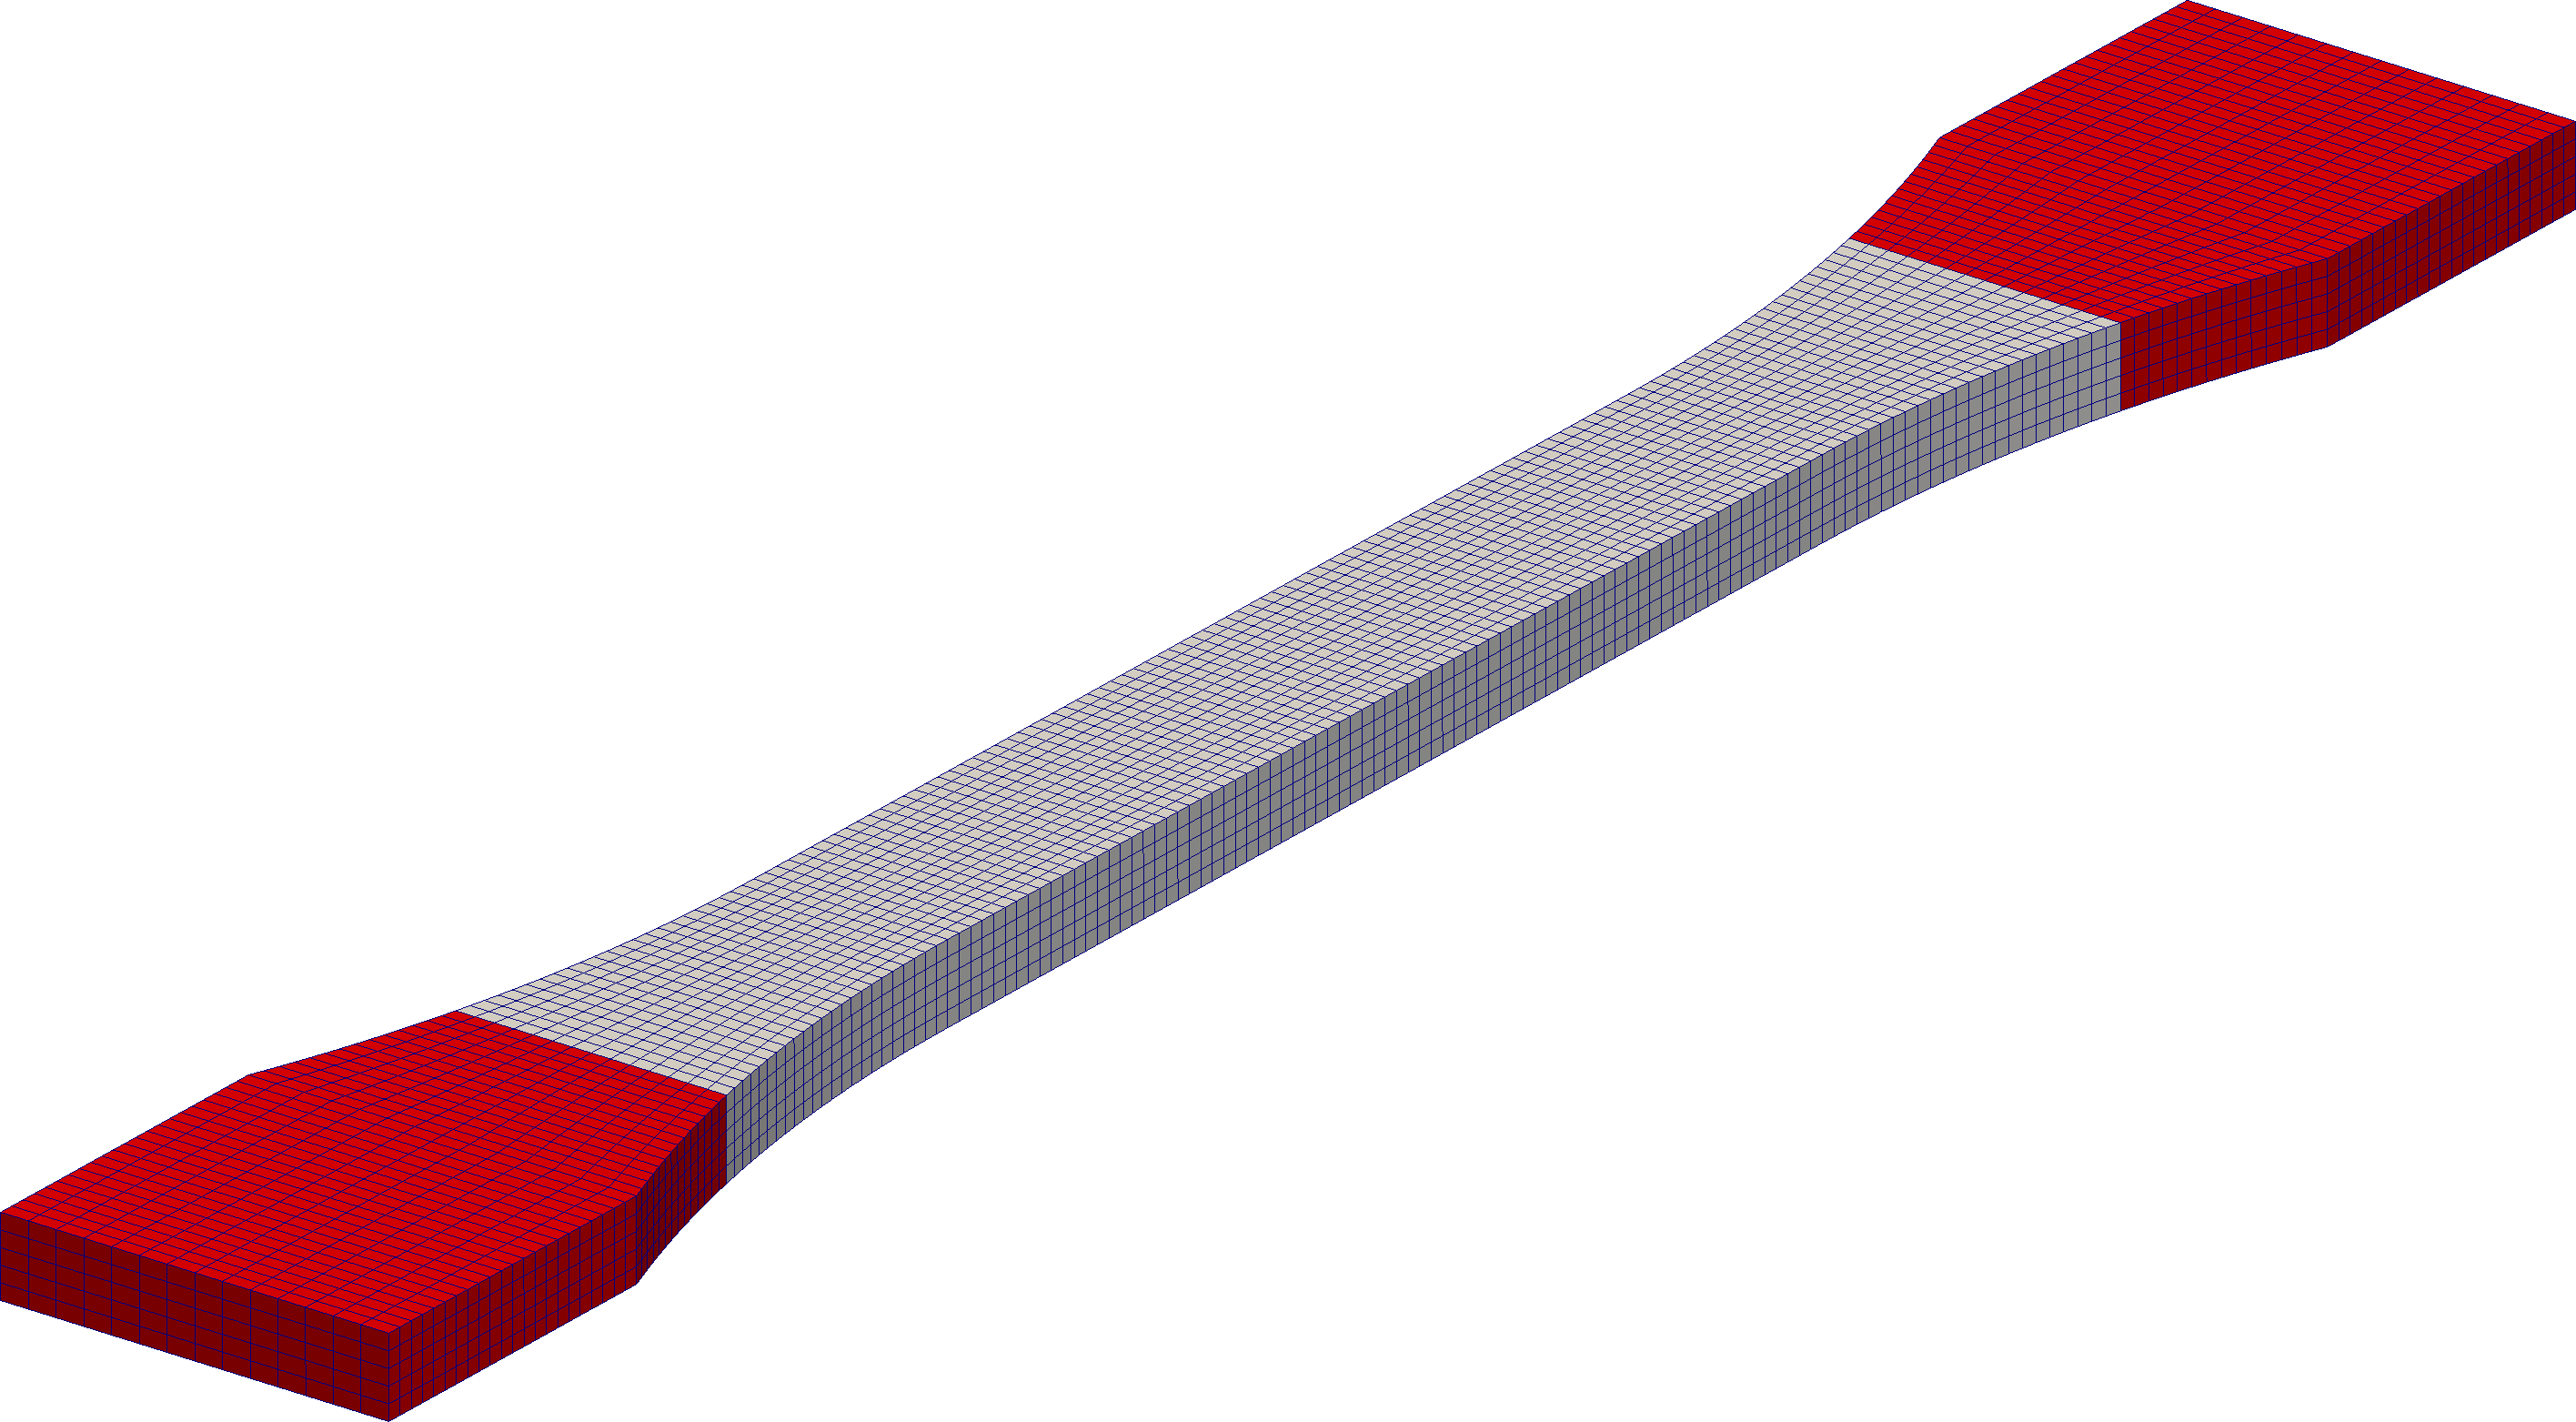
\includegraphics[width=\figwidth,height=\figheight,keepaspectratio]{Model_FE_Hex_0-4_ct}};
    \begin{scope}[
      shift={(FEHex.south west)},
      x={(FEHex.south east)},
      y={(FEHex.north west)},
    ]
      \coordinate (spypointfehex) at (0.8,0.715);
      \coordinate (spyviewerfehex) at (0.25,0.75);
      \spy on (spypointfehex) in node at (spyviewerfehex);
    \end{scope}
    
    \node[below right=\vsep and \hsep of sketch.east] (FETet) {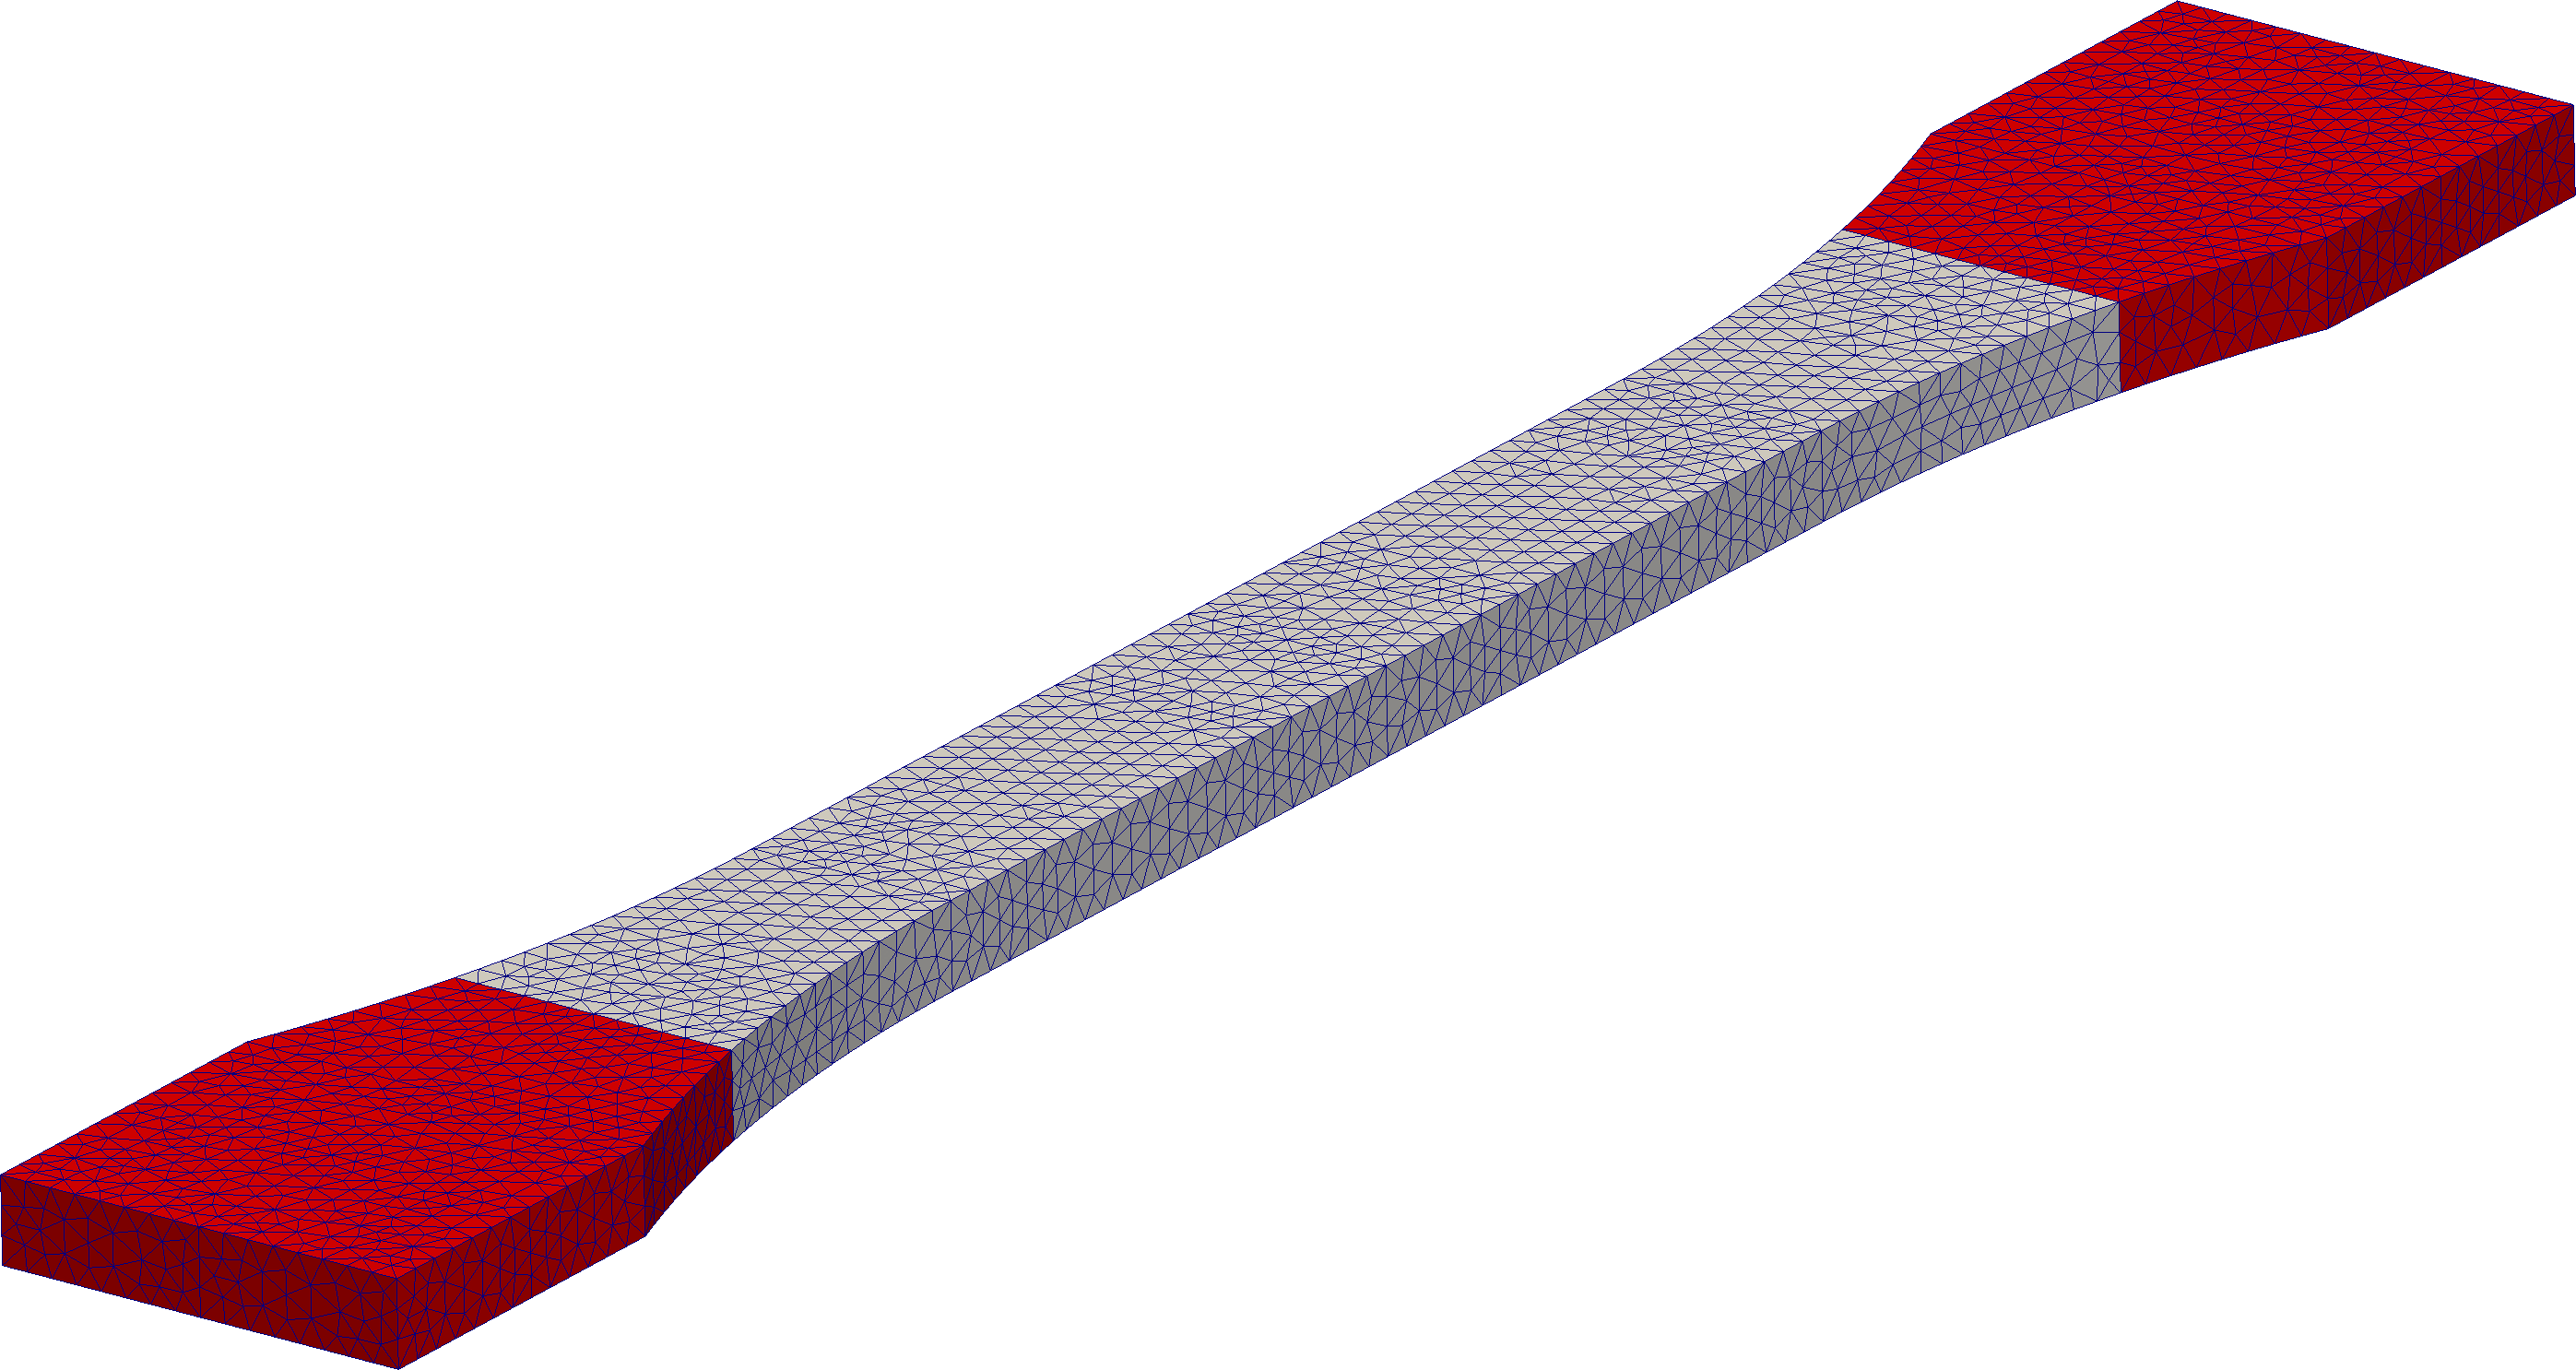
\includegraphics[width=\figwidth,height=\figheight,keepaspectratio]{Model_FE_Tet_0-67_ct}};
    \begin{scope}[
      shift={(FETet.south west)},
      x={(FETet.south east)},
      y={(FETet.north west)},
    ]
      \coordinate (spypointfetet) at (0.8,0.715);
      \coordinate (spyviewerfetet) at (0.25,0.75);
      \spy on (spypointfetet) in node at (spyviewerfetet);
    \end{scope}
    
    % PD
    \node[right=\hsep of FEHex.east,anchor=west] (PDHex) {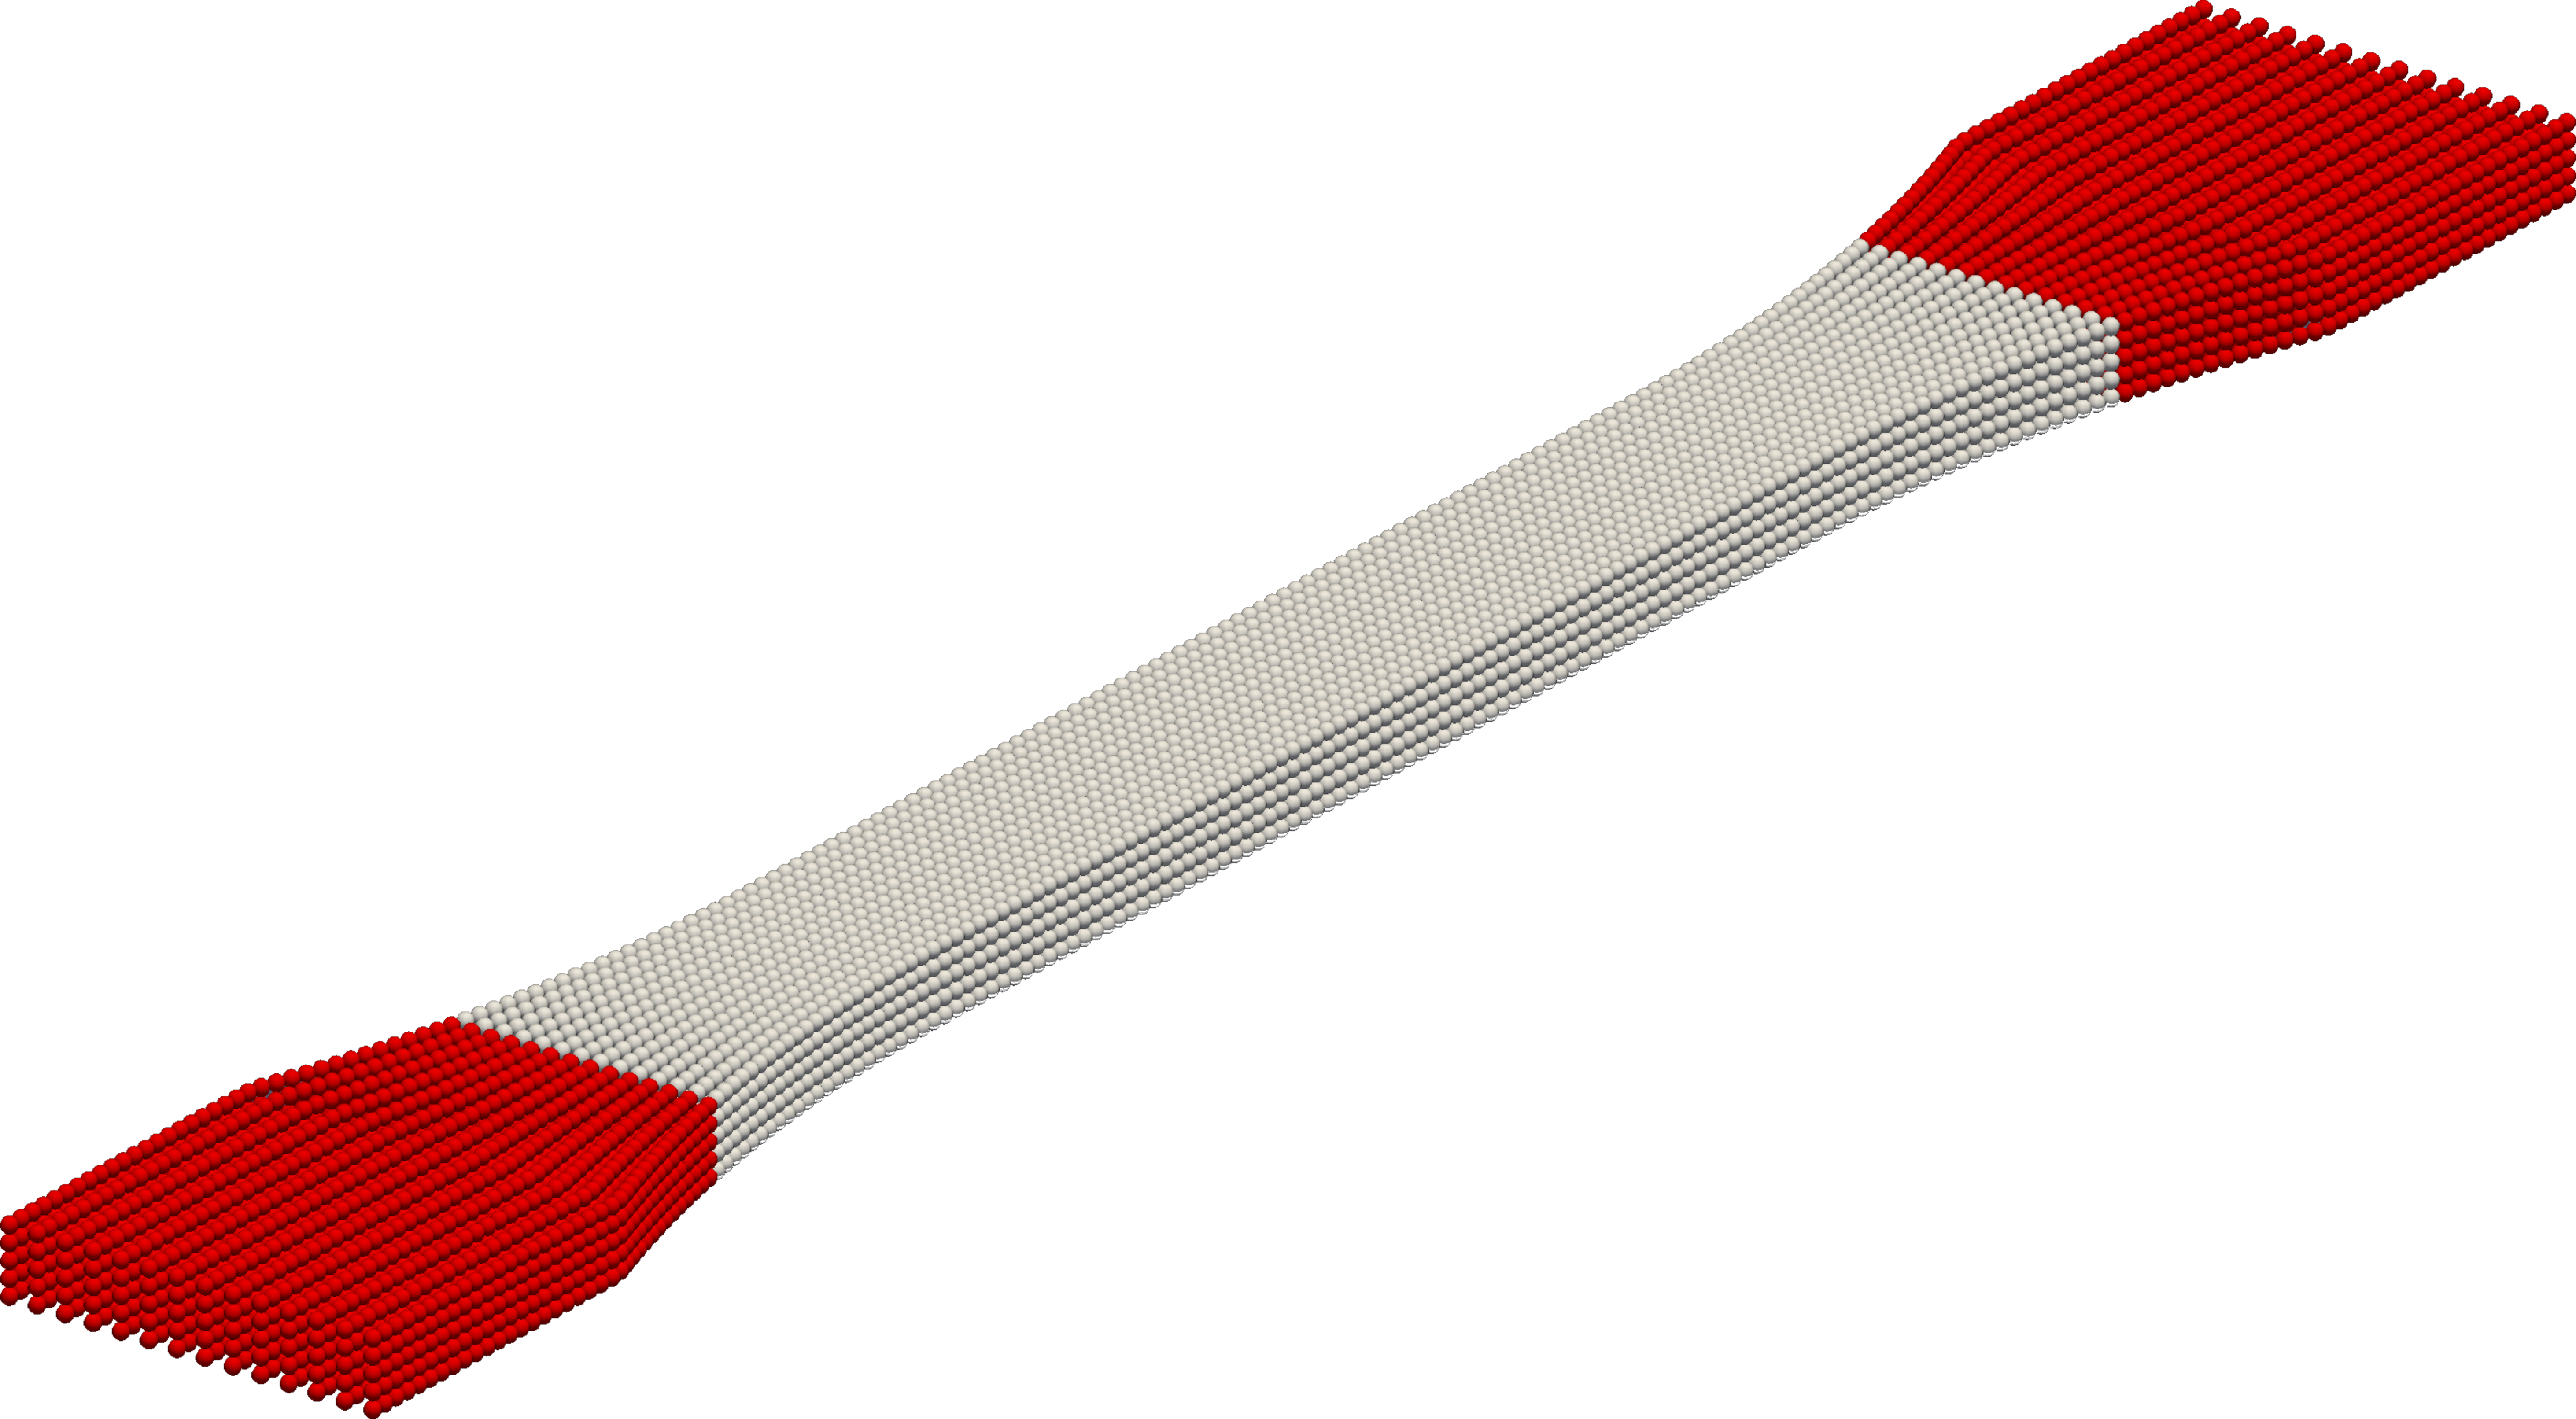
\includegraphics[width=\figwidth,height=\figheight,keepaspectratio]{Model_PD_Hex_0-4_ct}};
    \begin{scope}[
      shift={(PDHex.south west)},
      x={(PDHex.south east)},
      y={(PDHex.north west)},
    ]
      \coordinate (spypointpdhex) at (0.8,0.715);
      \coordinate (spyviewerpdhex) at (0.75,0.25);
      \spy on (spypointpdhex) in node at (spyviewerpdhex);
    \end{scope}
    
    \node[right=\hsep of FETet.east,anchor=west] (PDTet) {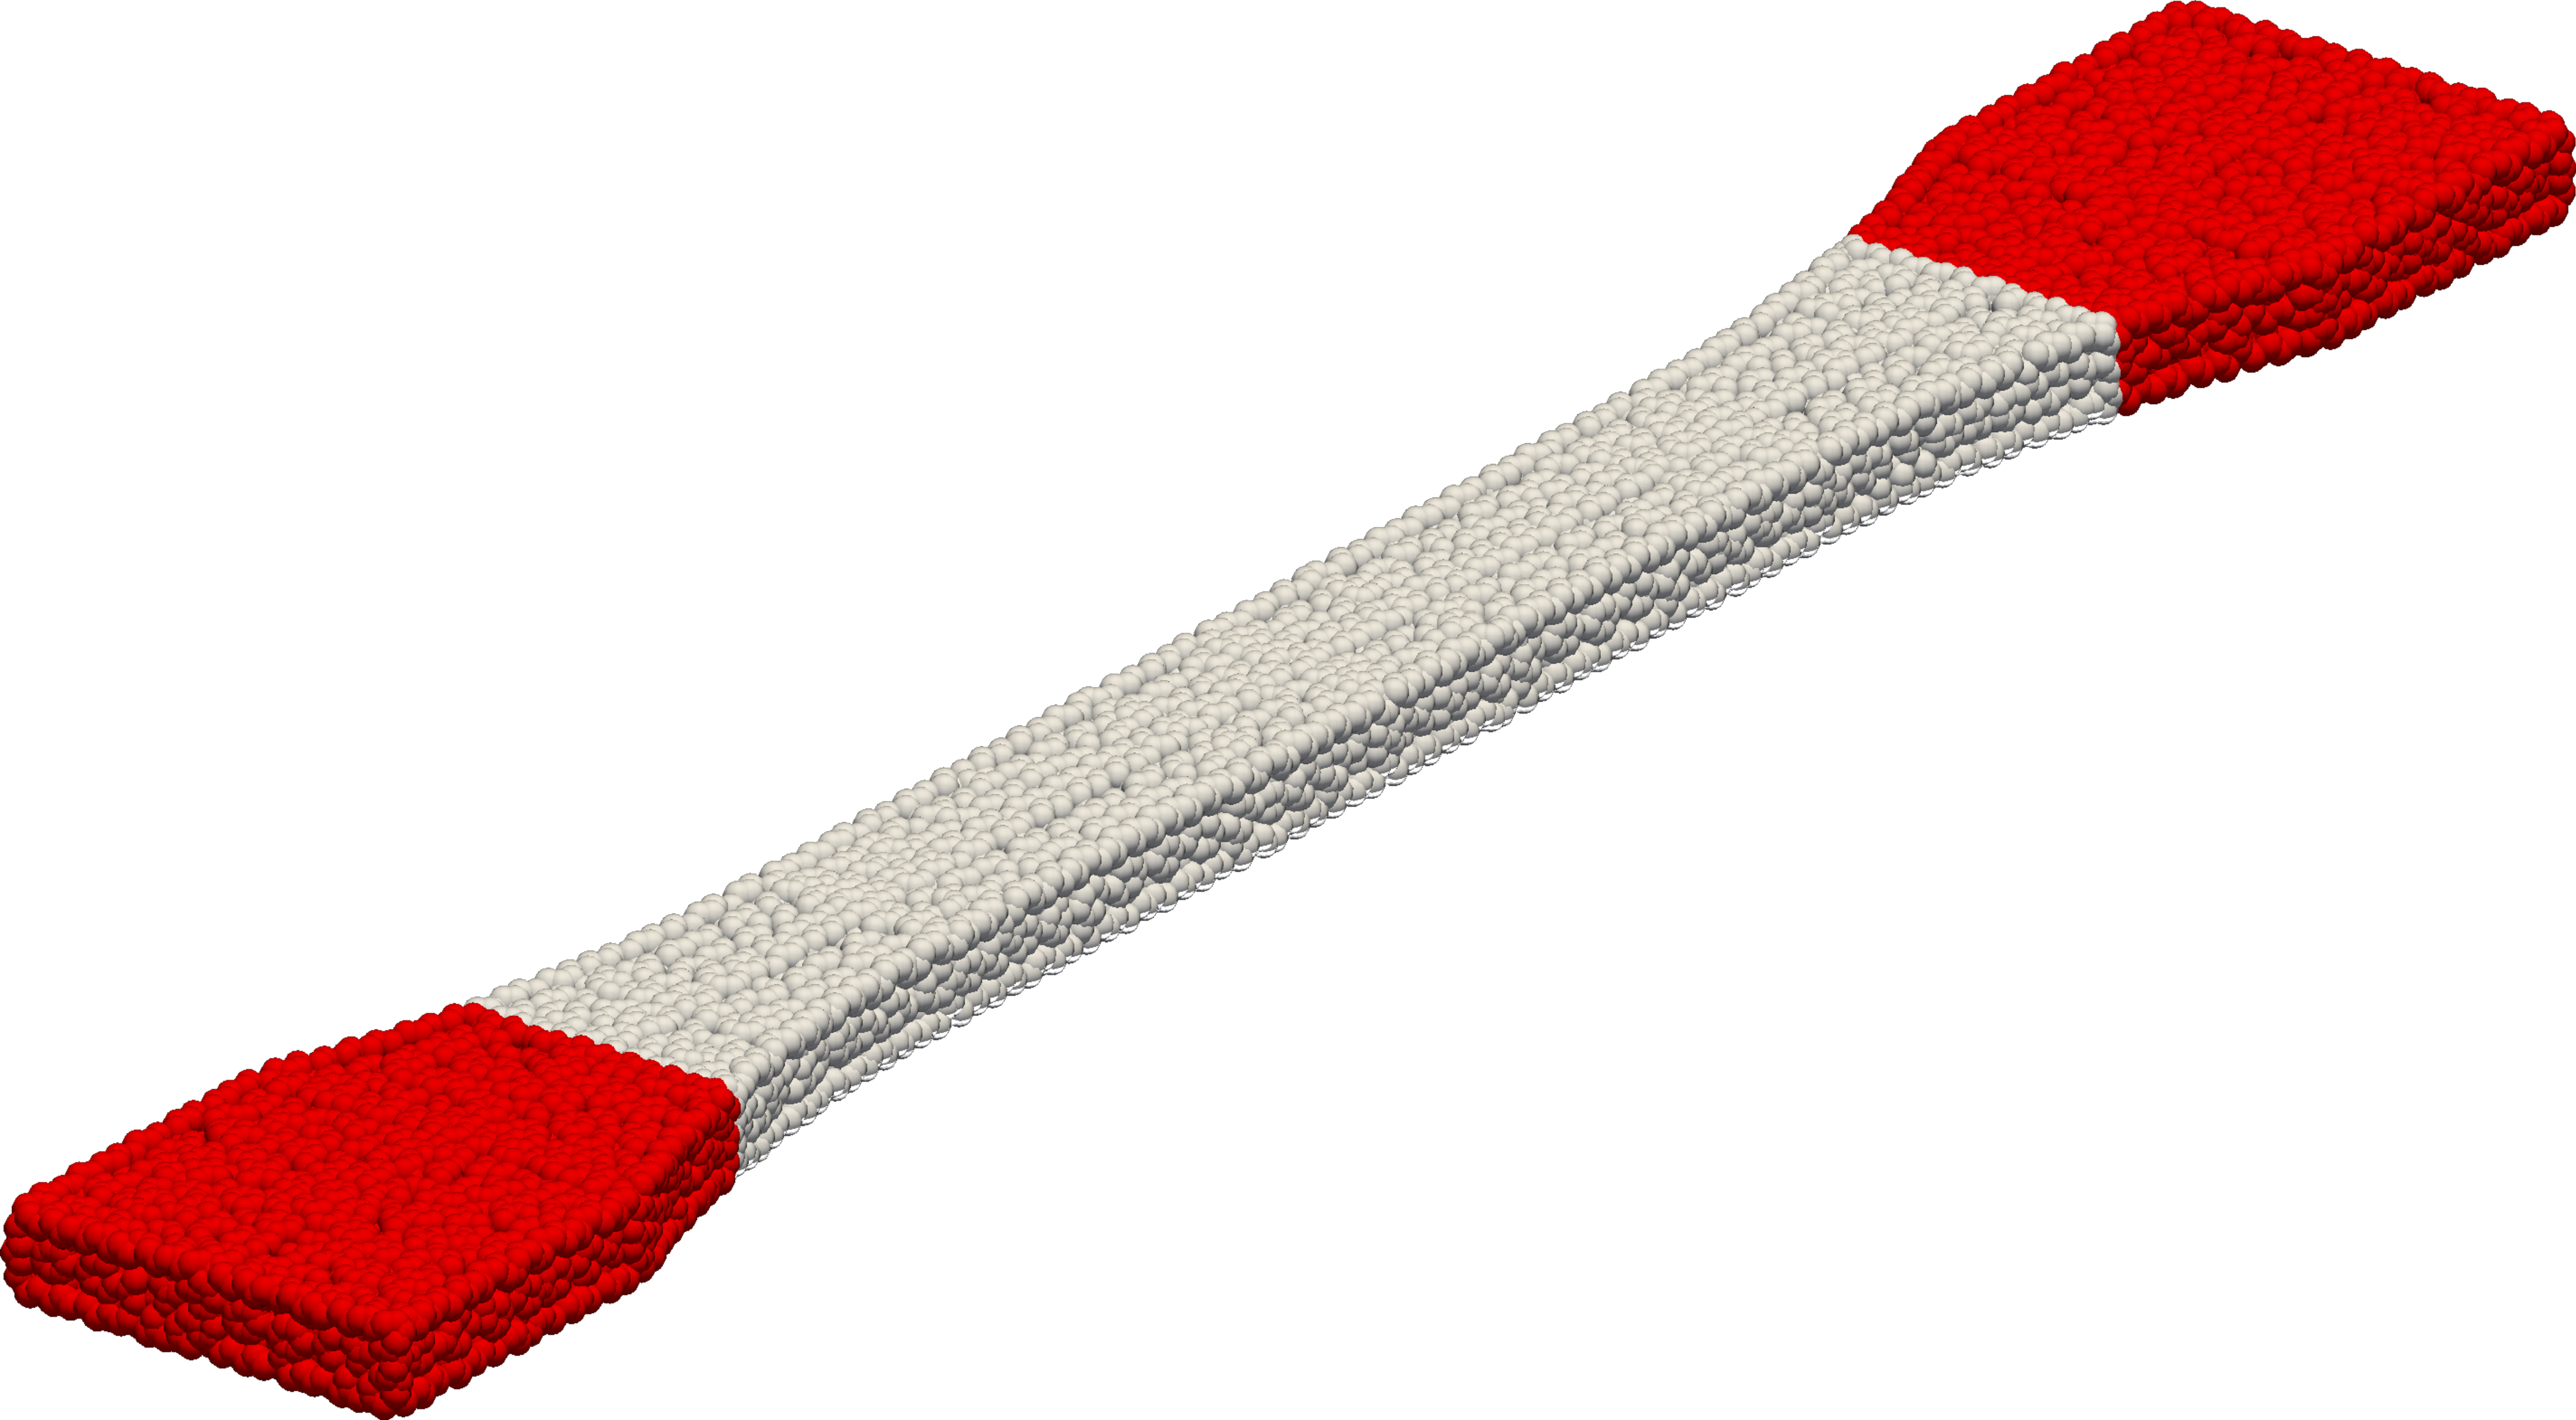
\includegraphics[width=\figwidth,height=\figheight,keepaspectratio]{Model_PD_Tet_0-67_ct}};
    \begin{scope}[
      shift={(PDTet.south west)},
      x={(PDTet.south east)},
      y={(PDTet.north west)},
    ]
      \coordinate (spypointpdtet) at (0.8,0.715);
      \coordinate (spyviewerpdtet) at (0.75,0.25);
      \spy on (spypointpdtet) in node at (spyviewerpdtet);
    \end{scope}
    
    % LBC
    \node[right=\hsep of PDHex.east,anchor=west] (LBCHex) {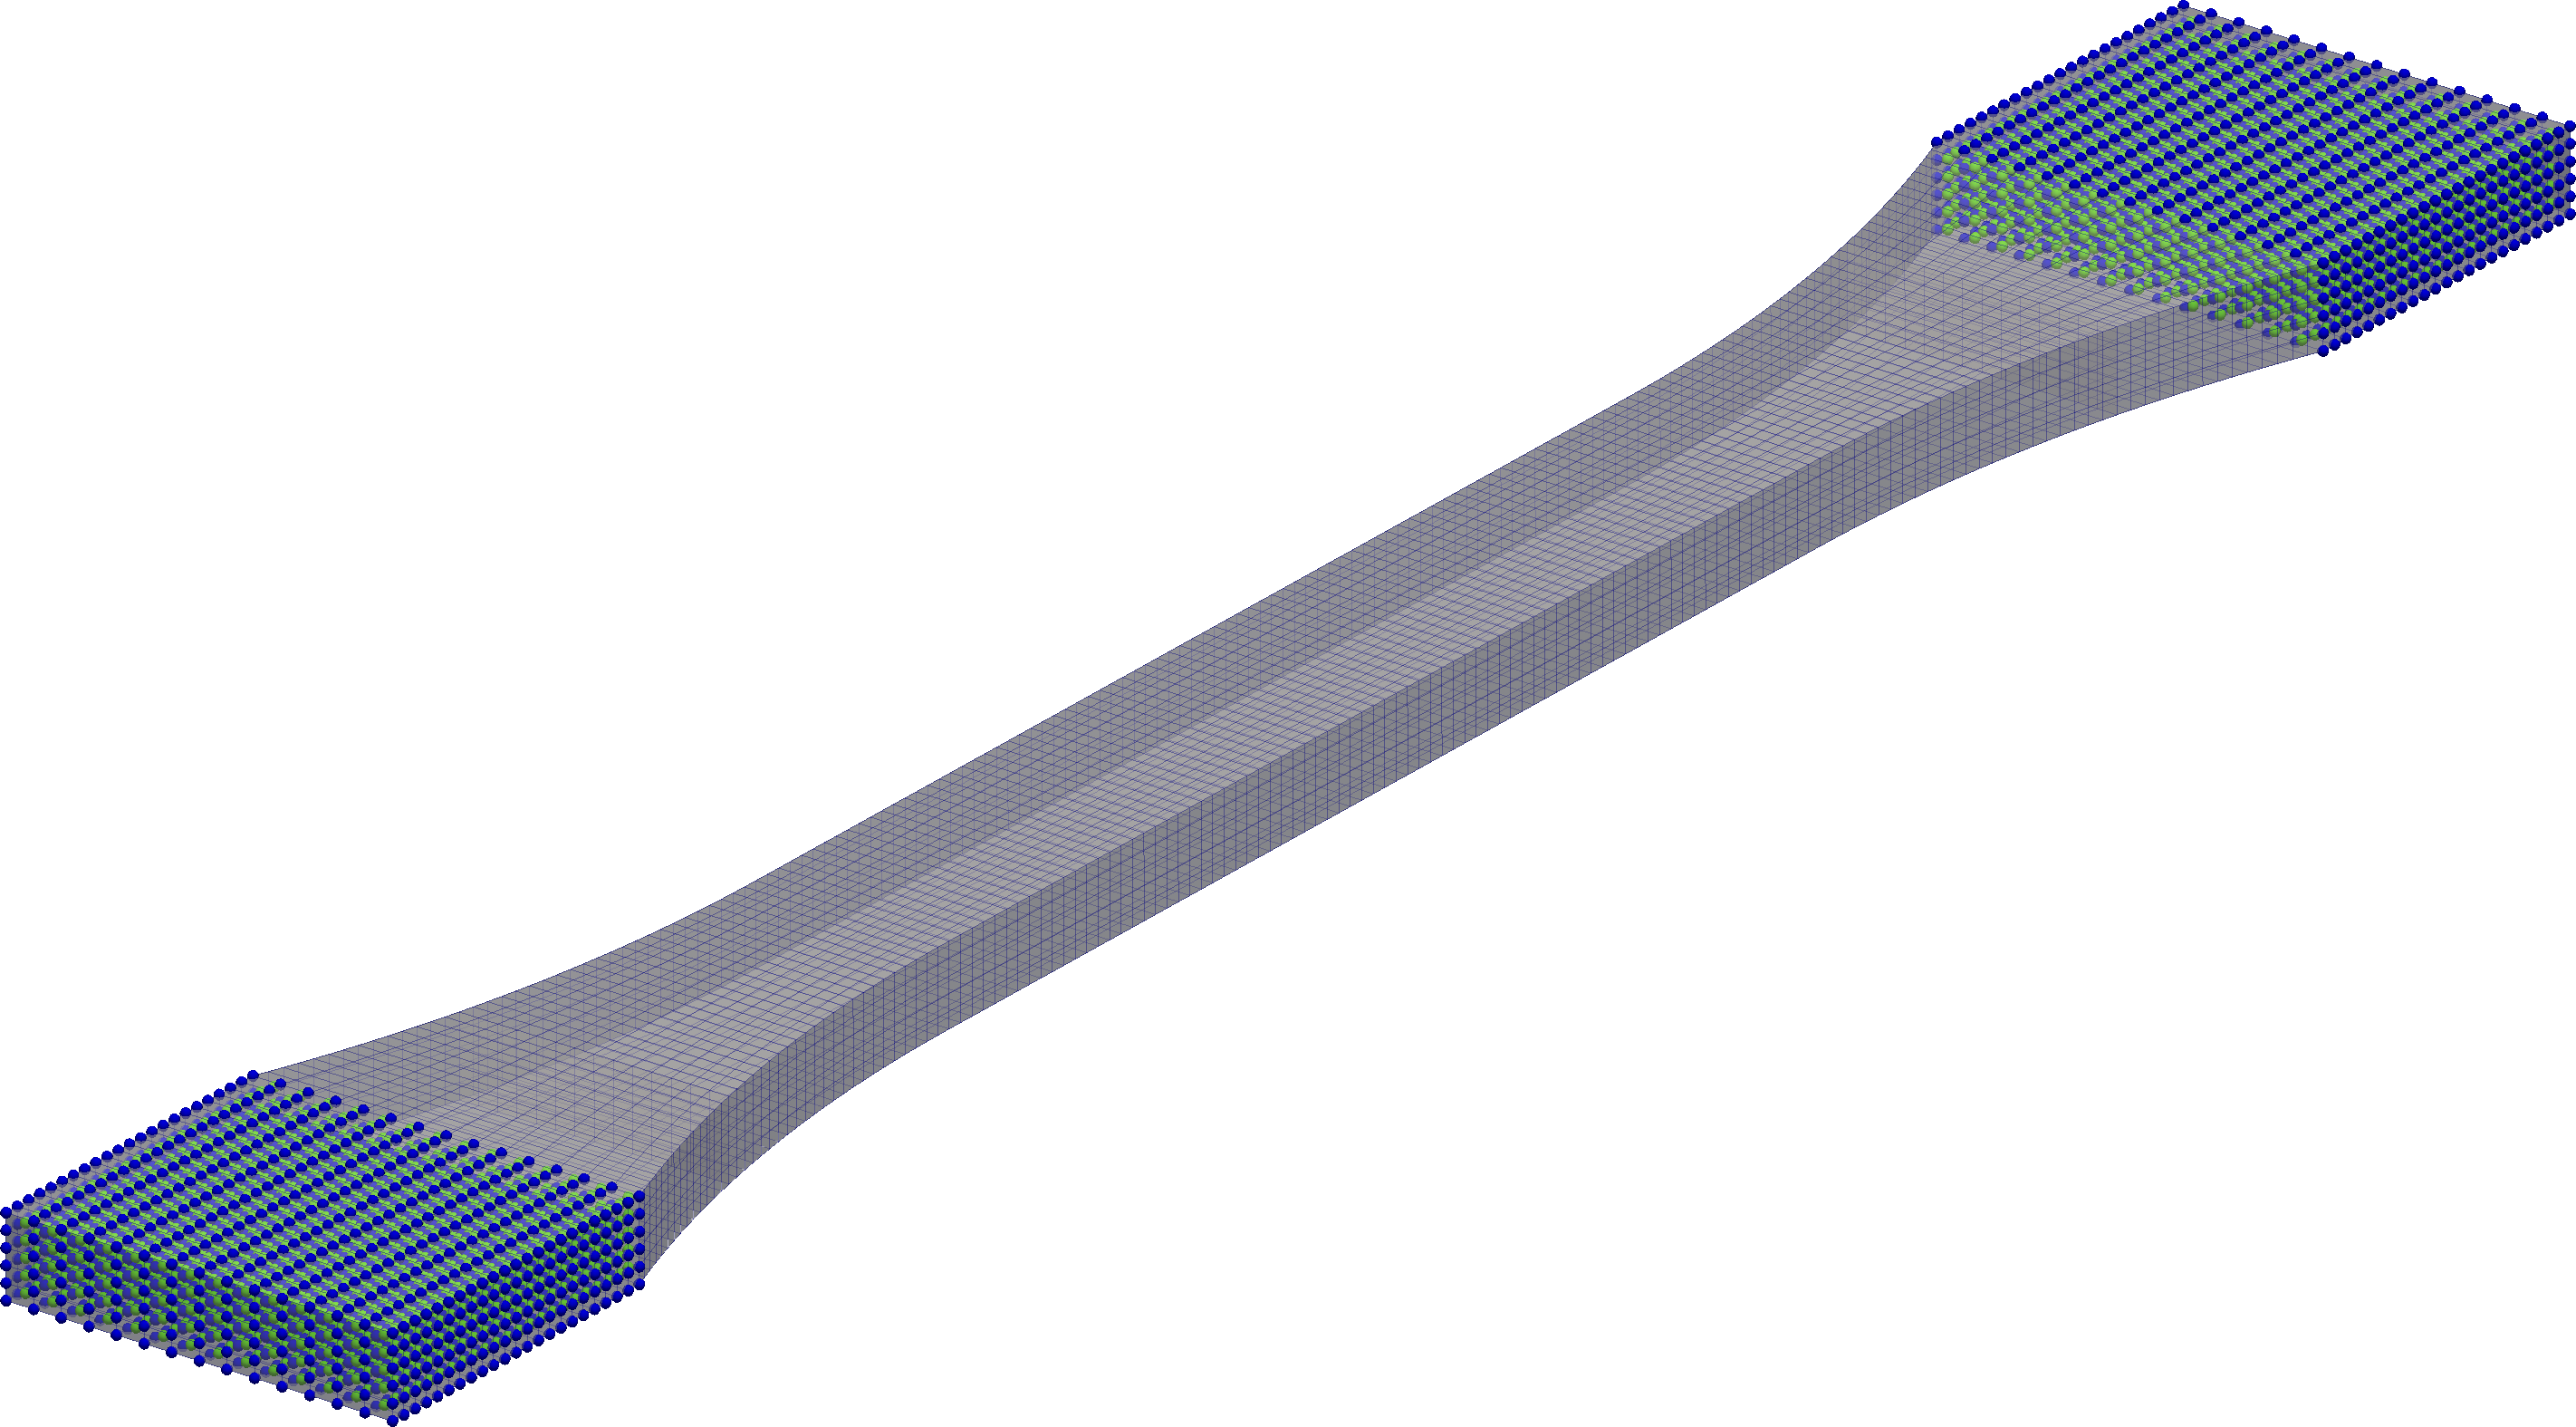
\includegraphics[width=\figwidth,height=\figheight,keepaspectratio]{Model_Mix_Hex_0-4_BC_NodeSets_Iso_ct}};
    \begin{scope}[
      shift={(LBCHex.south west)},
      x={(LBCHex.south east)},
      y={(LBCHex.north west)},
    ]
      \node (LBCHexDetail) at (0.80,-0.15) {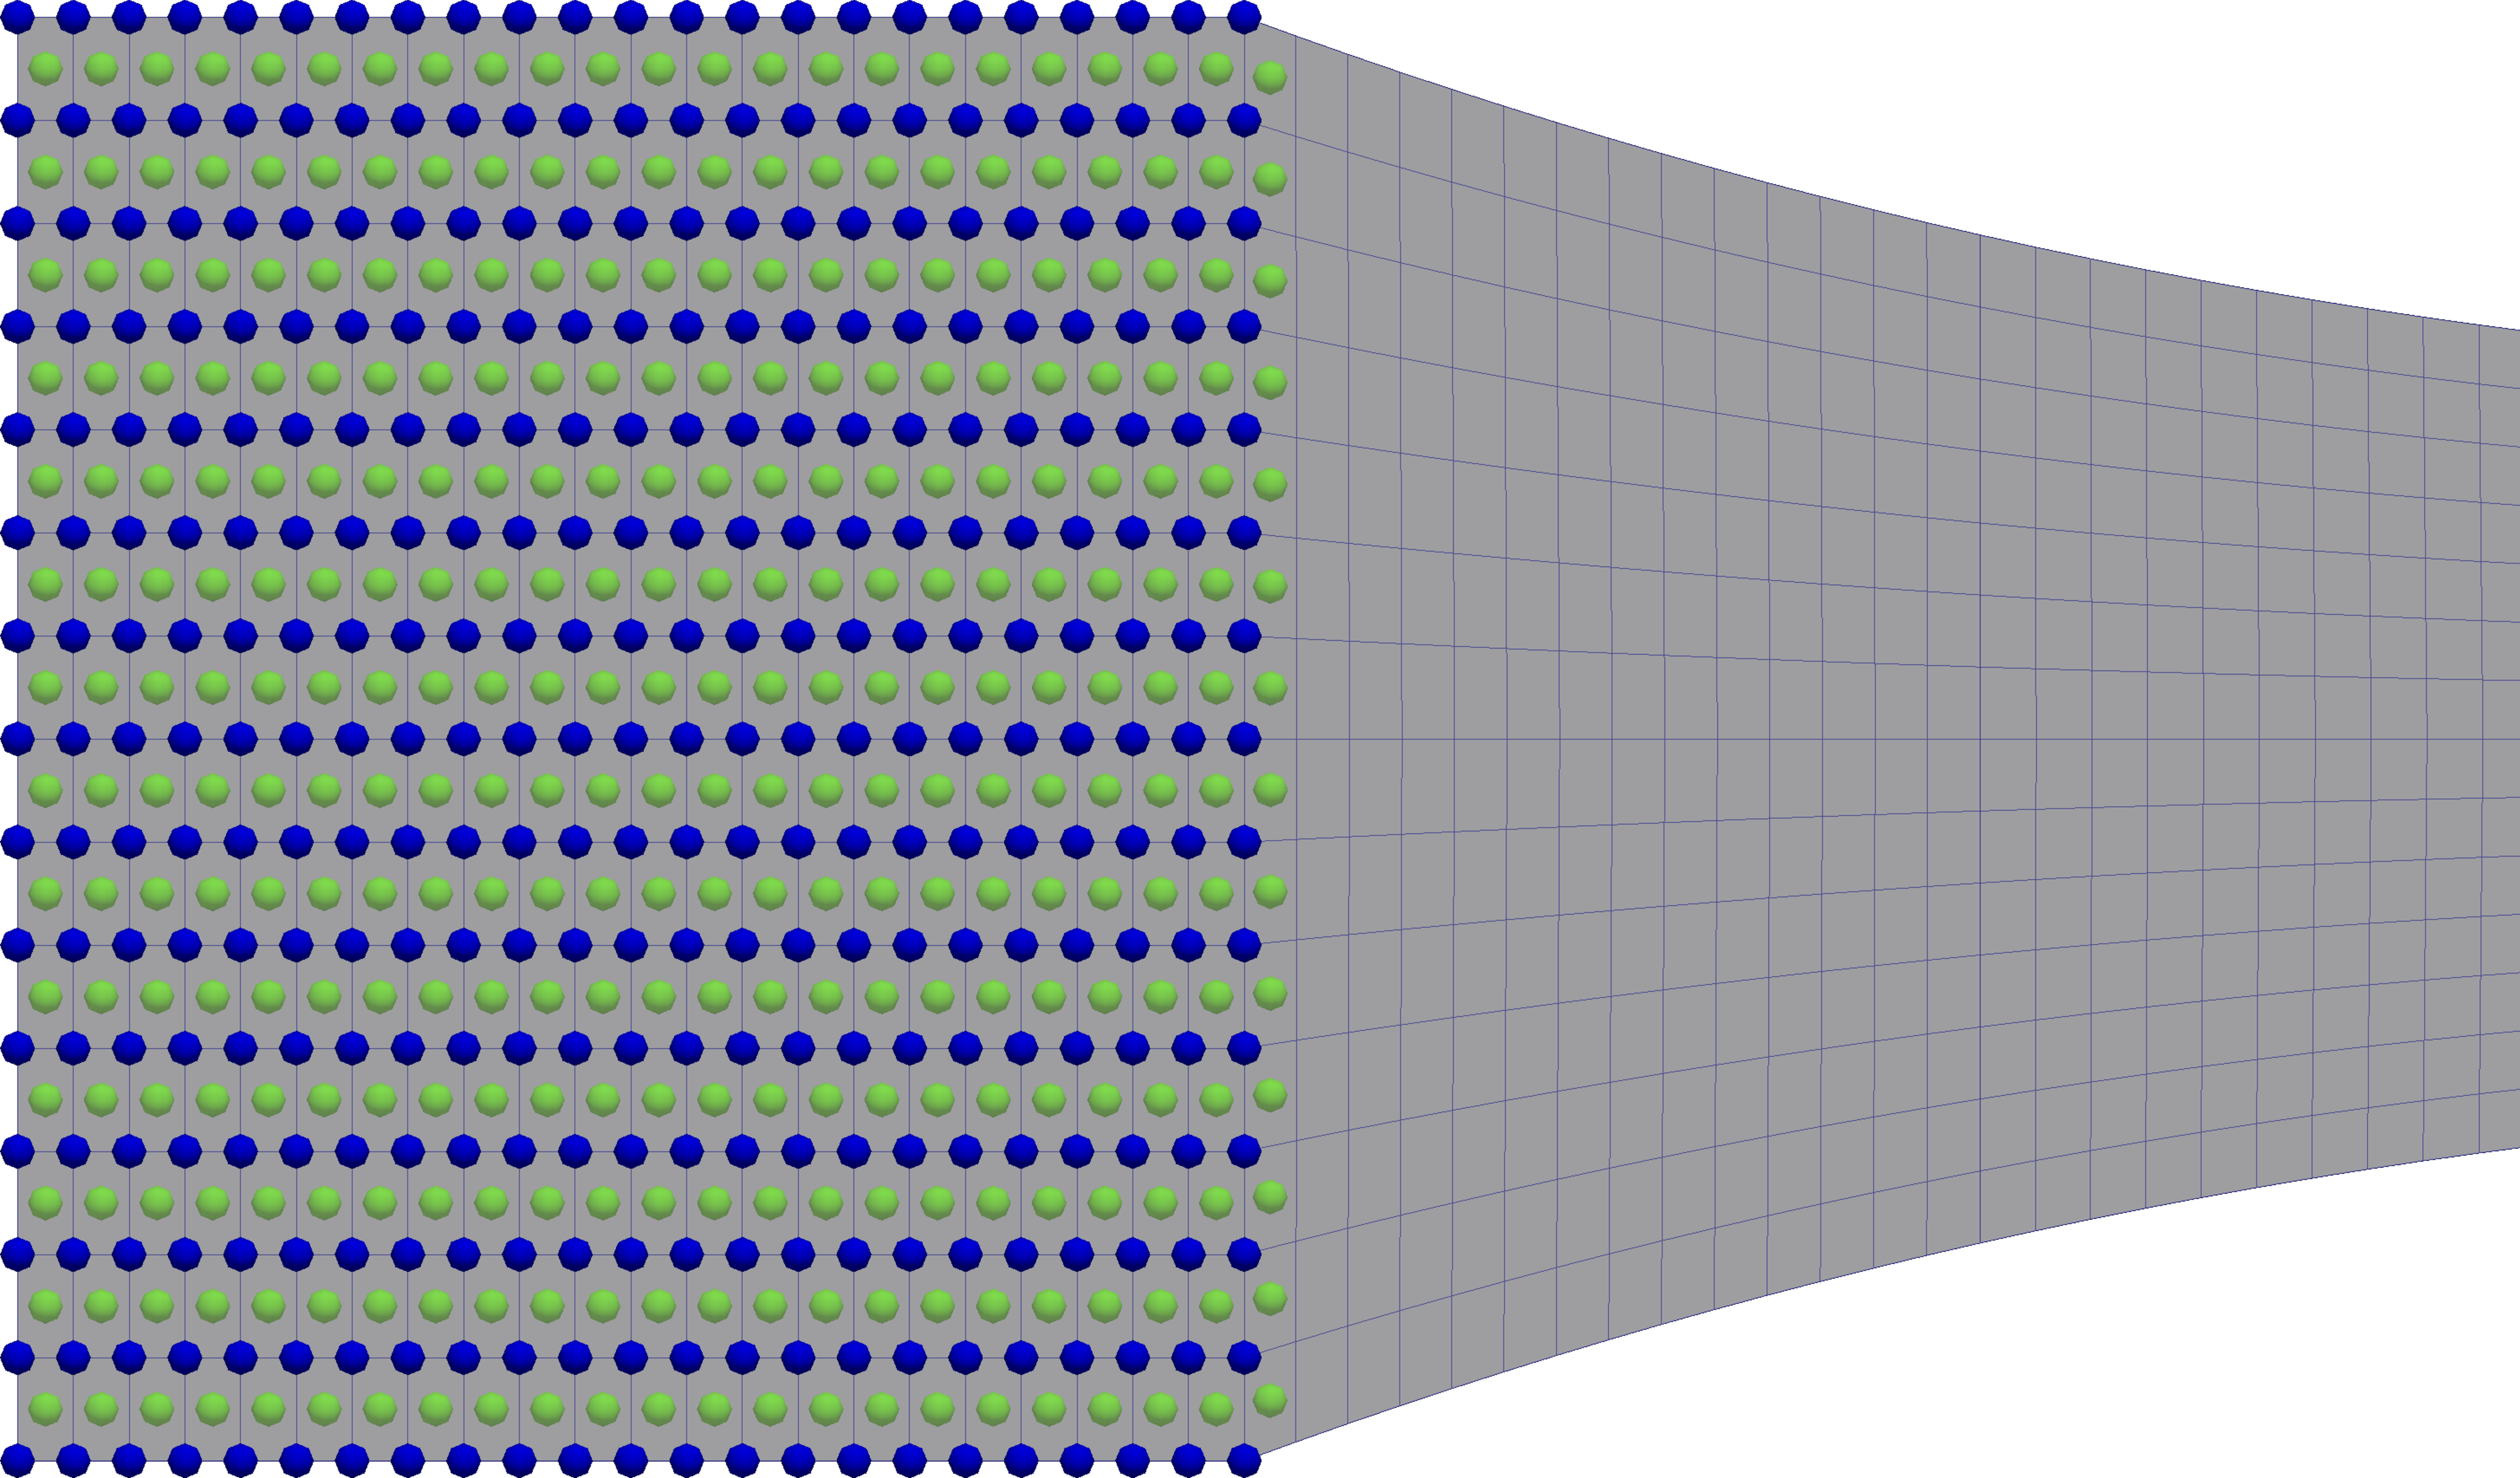
\includegraphics[width=0.20\linewidth,height=0.25\textheight,keepaspectratio]{Model_Mix_Hex_0-4_BC_NodeSets_ct}};
      %\coordinate (spypointlbchex) at (0.8,0.715);
      %\coordinate (spyviewerpdhex) at (0.75,0.25);
      %\spy on (spypointpdhex) in node at (spyviewerpdhex);
    \end{scope}
    
    \draw[-latex] (sketch) -- (FEHex) node[midway,above,sloped]{Hex};
    \draw[-latex] (sketch) -- (FETet) node[midway,below,sloped]{Tet};
    \draw[-latex] (FEHex)  -- (PDHex);
    \draw[-latex] (FETet)  -- (PDTet);
    \draw[-latex] (PDHex)  -- (LBCHex);
    
    \node[above=\vsep of  FEHex.north,anchor=south]{FE};
    \node[above=\vsep of  PDHex.north,anchor=south]{PD};
    \node[above=\vsep of LBCHex.north,anchor=south]{Loads \& BC};

  \end{tikzpicture}
  \endgroup
}

\end{frame}
